% Template for articles submitted to the International Journal of Forecasting
% Further instructions are available at www.ctan.org/pkg/elsarticle
% You only need to submit the pdf file, not the source files.
% If your article is accepted for publication, you will be asked for the source files.


\documentclass[11pt,3p,review,authoryear]{elsarticle}

\usepackage{listings}
\usepackage{color}
\usepackage{graphicx}
\usepackage{multirow}
\usepackage{array,rotating}
\usepackage{adjustbox}
\usepackage{numprint}
\usepackage{siunitx}
\usepackage{amsmath}


\definecolor{dkgreen}{rgb}{0,0.6,0}
\definecolor{gray}{rgb}{0.5,0.5,0.5}
\definecolor{dkred}{rgb}{0.6,0,0}

\lstset{frame=tb,
  language=R,
  aboveskip=3mm,
  belowskip=3mm,
  showstringspaces=false,
  columns=flexible,
  basicstyle={\small\ttfamily},
  numbers=none,
  numberstyle=\tiny\color{gray},
  keywordstyle=\color{blue},
  commentstyle=\color{dkgreen},
  stringstyle=\color{dkred},
  breaklines=true,
  breakatwhitespace=true,
  tabsize=3
}

\journal{International Journal of Forecasting}
\bibliographystyle{ijf}%model5-names}
\biboptions{longnamesfirst}
% Please use \citet and \citep for citations.


\begin{document}

\begin{frontmatter}

\title{Fast and Accurate Yearly Time Series Forecasting with Forecast Combinations}

%% AUTHORS %%%%%%%%%%%%%%%%%%%%%%%%%%%%%%%%%%%%%%%%%%%%%%%%%%%%%%%%%%%%%%%%%%%%
%% Leave this section commented out so that the paper is blinded for review.
%% Group authors per affiliation:
\author[ss]{David Shaub\corref{cor}}
\address[ss]{Harvard University Extension School}


%% Only give the email address of the corresponding author
\cortext[cor]{Corresponding author}
\ead{davidshaub@g.harvard.edu}
%%%%%%%%%%%%%%%%%%%%%%%%%%%%%%%%%%%%%%%%%%%%%%%%%%%%%%%%%%%%%%%%%%%%%%%%%%%%%%%%


\begin{abstract}
It has long been known that combination forecasting strategies produce superior out-of-sample forecasting performances. In the M4 forecasting competition, a very simple forecast combination strategy achieved third place on yearly time series. An analysis of the ensemble model and its component models suggests that the competitive accuracy comes from avoiding poor forecasts, rather than from beating the best individual models. Moreover, the simple ensemble model can be fitted very quickly, can easily scale horizontally with additional CPU cores or a cluster of computers, and can be implemented by users very quickly and easily. This approach might be of particular interest to users who need accurate yearly forecasts without being able to spend significant time, resources, or expertise on tuning models. Users of the R statistical programming language can access this modeling approach using the ``forecastHybrid'' package.
\end{abstract}

\begin{keyword}
Automatic forecasting\sep Combining forecasts\sep Evaluating forecasts\sep Forecasting competitions\sep Software
% Suggested keywords are listed at https://ijf.forecasters.org/keywords/
\end{keyword}

\end{frontmatter}


\section{Introduction}
Model selection presents a challenge for forecasters, since model specification error leads to additional forecasting error. Combining several candidate models can hedge against an incorrect model specification. \cite{BatesGranger1969} suggested such an approach and observed, somewhat surprisingly, that the combined forecast can even outperform the single best component forecast. While combination weights that are selected equally or proportionally to past model errors are possible approaches, many more sophisticated combination schemes have been suggested. For example, rather than normalizing weights to sum to unity, unconstrained and even negative weights could be possible \citep{GrangerRamanathan1984}.

\cite{HIBON2005} investigate the tradeoff between combing worse component forecasts and the risk of incorrect model selection, and find that, while the best individual model and the combination perform equally well, the combination protects against the very large misses that can occur with model selection. A simple mean combination of forecasts is sensitive to extreme values, so trimmed mean procedures have been suggested and have been shown to reduce extreme errors \citep{JOSE2008}. For a more complete history of the forecast combination literature, including contributions outside the field of economics such as psychology and management science, see \cite{CLEMEN1988}.

The simple equal-weights combination might appear woefully obsolete and probably noncompetitive compared to the multitude of sophisticated combination approaches or advanced machine learning and neural network forecasting models, especially in the age of big data. However, the results from the 2018 M4 competition \citep{M4} show that such simple combinations can still be competitive, particularly for yearly time series, where the method achieved third place. This paper therefore seeks to examine why such a simple combination procedure remains effective and proved competitive in the M4 competition when pitted against more sophisticated models. Specifically, it seeks to contribute to our understanding of how simple model combinations perform relative to in-sample and oracle model selection procedures.

This article is organized as follows: Section 2 describes the combination methodology, Section 3 contains an analysis of the performance characteristics of this model in the M4 competition relative to individual models, and Section 4 concludes.


\section{Methodology}
The author's submission to the M4 competition utilized this combination strategy only for the yearly time series, with a temporal hierarchical approach using the ``thief'' R package \citep{ATHANASOPOULOS201760} being used for the other frequencies (i.e., hourly, daily, weekly, monthly, quarterly). As a result, the scope of the analysis in this paper will be limited to the performance of the combination strategy on the yearly time series in the M4 competition.

The combination strategy employed in the M4 competition submission employed the statistical programming language R \citep{Rlang} and made use of the ``forecastHybrid'' \citep{forecastHybrid} package. The component models allowed in the ``forecastHybrid'' package are the \texttt{auto.arima} (automatic selection of AR, MA and the integration order for seasonal time series), \texttt{ets} (exponential smoothing with automatic selection of the additive/additive damped/multiplicative/multiplicative damped trend and seasonal components), \texttt{thetaf} (the Theta model described by \citealp{THETA}), \texttt{nnetar} (a feedforward neural network with lags as features), \texttt{stlm} (a simple
seasonal and trend decomposition), \texttt{tbats} (a state space model with Box-Cox transforms for handling scale invariance, Fourier transforms for handling complex and time-varying seasonality, and ARMA for error correction, as described by \cite{TBATS}), and \texttt{snaive} (a seasonal na\"ive forecast). All of these models are provided by the ``forecast'' package \citep{Forecast}. The ``forecastHybrid'' package includes these component models in order to enhance the ``forecast'' package base models with easy ensembling.

The ``forecastHybrid'' package produces forecasts out to a horizon $h$ by applying a weight $w_m$ to each $m$ of the $n$ model forecasts in the ensemble. The ensemble forecast $f(i)$ for time horizon $1 \leq i \leq h$ and with individual component model forecasts $f_m(i)$ is then
\begin{align}
f(i) & = \sum_{m=1}^n w_m\cdot f_m(i).
\end{align}
The weights can be determined in several ways (for example: supplied by the user, set equally, determined by in-sample errors, or determined by cross-validation). Although this is not a requirement, the weights will sum to unity for all weight modes except when supplied by the user. For the M4 submission, the weights were set equally and automatically to $w_m = \frac{1}{n} = \frac{1}{3}$, since this method is the quickest. Perhaps surprisingly, this simple average was enough to be competitive.

For the author's submission to the M4 competition, only the \texttt{auto.arima}, \texttt{thetaf}, and \texttt{tbats} component models were included in the yearly ensemble.\footnote{This R function will produce point forecasts for an input time series \texttt{x} with a forecast horizon \texttt{h} using the three component models: \texttt{forecastM4 <- function(x, h = 6) forecast(hybridModel(x, models = "aft")}.} These models were selected from the author's experience, as they tend to produce reasonable forecasts for a wide range of time series behaviors; furthermore, they can capture can capture both seasonal and nonseasonal dynamics in the data generating process and have reasonable selection procedures that prevent the drastic overfitting that can occur for models with too many free coefficients. Moreover, performance was a concern, since the M4 competition required a large number of time series to be forecast with prediction intervals. In particular, the \texttt{nnetar} model could not be included, despite its favorable ability to handle nonlinear properties in the time series, since its empirical simulations for the prediction intervals are quite slow. The \texttt{ets} model was not included because the \texttt{tbats} and \texttt{auto.arima} models should be able to capture any data generating process that the state space model handles well. Finally, the \texttt{stlm} seasonal decomposition was also deemed unnecessary, since the author expected many structural breaks in the M4 time series that would not be handled well, and the \texttt{snaive} model was also deemed too simple to be competitive with machine learning techniques that could be used to learn across the 100,000 time series.


The forecasting procedure can be parallelized to decrease the time taken to fit models. A user can apply this parallelization both within models and across time series. If a single time series needs to be fitted, the three individual component models can be fitted in parallel on a separate CPU core/thread by passing the \texttt{parallel = TRUE} argument to the \texttt{hybridModel()} function; the \texttt{auto.arima} and \texttt{tbats} models themselves can also use parallel processing.\footnote{For a more detailed description of the ``forecastHybrid'' package and its usage, refer to the package vignette at https://cran.r-project.org/web/packages/forecastHybrid/vignettes/forecastHybrid.html or the package reference manual at https://cran.r-project.org/web/packages/forecastHybrid/forecastHybrid.pdf.} Furthermore, when users need to fit a model and forecast many time series (such as in the case of M4's 23,000 yearly time series), this forecasting function can be run as a distributed map operation on multiple CPUs or machines in a cluster. For example, if we wish to utilize 16 threads on a server to forecast the M4 time series in a list \texttt{M4Yearly}, we could use the ``pbapply'' package \citep{pbapply} to map the forecasting task and also to view a real-time progress bar with an estimated completion time.\footnote{The following R code will use 12 processes/threads to forecast a list \texttt{M4Yearly} of yearly time series in parallel: \texttt{forecasts <- pblapply(M4Yearly, forecastM4, cl = 12)}.} The training and forecasting process is fast: on an i7-8850H CPU with 6 cores and 12 threads, the entire training and forecasting procedure takes approximately 55 minutes for the 23,000 yearly M4 time series, which is about seven time series per second.


This parallelization strategy was used in our M4 submission, and the entire setup of the R environment, the installation of dependencies packages, and the download of the M4 dataset were packaged into a Docker container for reproducibility. The simplicity of this approach offers considerable flexibility to practitioners who need to adjust the latency of model training and forecasting without writing much custom or complex code. Indeed, the author's M4 submission for all time series amounted to fewer than 100 lines of R code and did not employ prepossessing or filtering, which can make the deployment of automated forecasting systems at scale in a production environment difficult and vulnerable to the use of new and degenerate datasets with characteristics such as missing data, extreme values, zero variances, etc. Modeling approaches that require the building of features or training across time series may not be so readily applicable online or so amenable to an ``embarrassingly parallel'' workflow or an easily-tunable user selection as to whether to apply parallelization within models or across time series. This approach is therefore of interest to those who need a fast and tunable system to run at scale.


\section{Analysis}
We might reasonably question why such a simple and well-known technique of averaging forecasts proved competitive in the M4 yearly time series. One hypothesis is that model selection is a difficult problem, and more complex forecasting methodologies struggle to select a model that will perform well on out-of-sample data. The model selection problem for complex models could manifest itself as either explicit selection from a pool of candidate models (or of the weights assigned to these models if using more than one) or the implicit problem of selecting the optimal coefficients if a single, complex model with many free variables is used. The examination that follows supports this hypothesis and shows that the mean ensemble approach achieves a competitive performance not by producing forecasts that barely miss the actual values, but rather by producing fewer forecasts that miss the actual values very badly.


We examine three separate modeling strategies here. The first is the ensemble approach that was used in the M4 submission and described in Section 2. The second is a model selection procedure that attempts to choose the single best model for the forecasting period based on the individual model that performs best on a holdout set created from the M4 training data. Since the M4 forecasting horizon for the yearly data is six, the final six observations of a time series are removed and each individual component model (\texttt{auto.arima}, \texttt{thetam}, and \texttt{tbats}) is estimated on the truncated training time series. Each model then forecasts against the six observations, and the best individual model based on the mean absolute scaled error (MASE) is selected and retrained on the full, original time series. If multiple models have equivalent minimum MASE values (as happens for constant, linear trend, or other time series that each model can predict perfectly on the holdout set), a single component model is selected at random from those with the best MASE. The third and final model for comparison is a reference oracle model that is the individual component model for each time series that performs best on the M4 competition evaluation set. This final model is built not as a legitimate contender for a modeling strategy that could be used in practice for forecasting, but rather to evaluate the efficacy of the second model selection procedure and as a benchmark for comparing the accuracy of our forecasts against the best that we might hope to do in some sense, at least with a single component model from the set of candidate models that we examine here.


% Distribution of log(MASE) for ensemble and selected models
\begin{figure}[h]
\centering
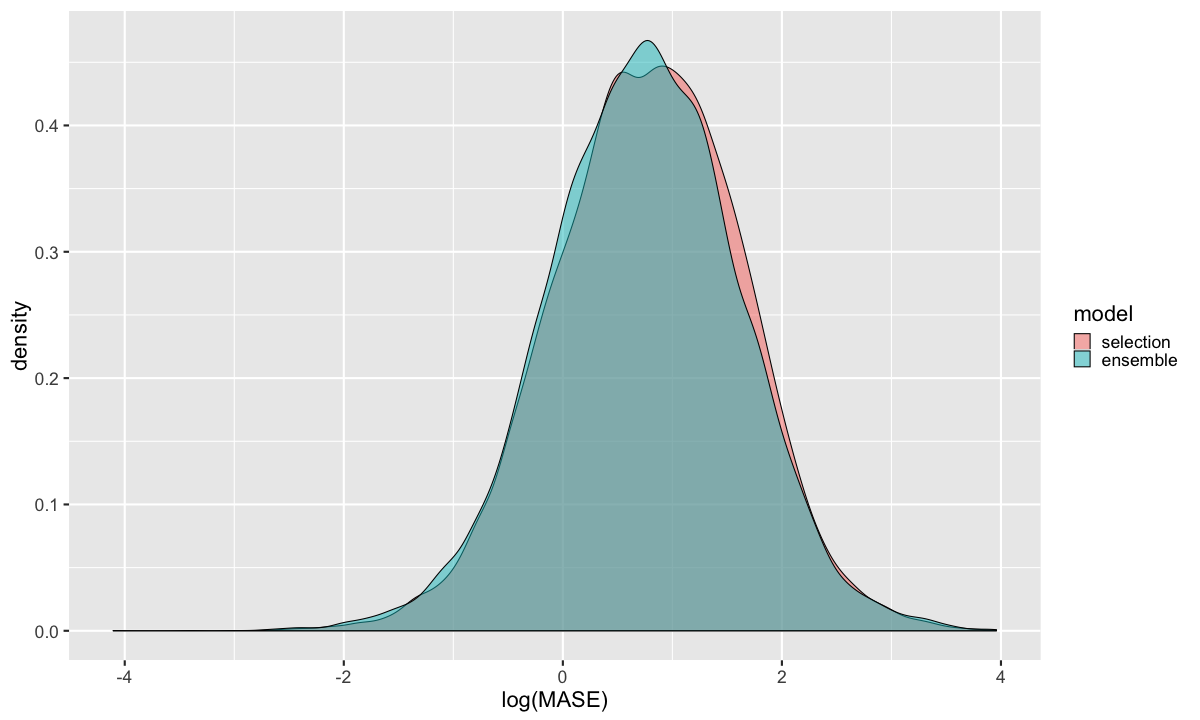
\includegraphics[width=\textwidth]{distribution}
\caption{Distribution of MASE values for the ensemble and model selection forecasting procedures.}\label{fig:a}
\end{figure}

% Table distribution of MASE for ensemble, oracle, and selection
\begin{table}[ht]
\centering
\caption{MASE summary statistics for the oracle reference, selection, and ensemble models.}\label{tab:a}
\npdecimalsign{.}
\nprounddigits{3}
\begin{tabular}{rcccccc}
\hline
& Min & 1st quartile & Median & Mean & 3rd quartile & Max\\
\hline
Reference \vline & 0.000 & 0.852 & 1.503 & 2.275 & 2.669 & 51.521\\
Selection \vline & 0.000 & 1.235 & 2.224 & 3.133 & 3.953 & 51.521 \\
Ensemble \vline & 0.0505 & 1.170 & 2.104 & 3.039 & 3.722 & 52.414\\
\hline
\end{tabular}
\end{table}


Table~\ref{tab:a} and Figure~\ref{fig:a} show the distribution of MASE for the models. In particular, we can see that the ensemble model produces fewer forecasts with larger MASE values than does the selection procedure; the benefit appears to be most noteworthy between the second and third quartiles. However, both of these approaches fall far short of the oracle reference model, indicating that we could expect substantial improvements in forecasting accuracy over the ensemble method if a model selection procedure could achieve high levels of sensitivity and accuracy in selecting the correct model.


The model selection procedure employed here performs poorly; in fact, it is worse than the naive approach of using the dominant class Theta model for every time series without bothering to evaluate its performance on a holdout set. To be fair, when constructing forecasts, a forecaster would not know \textit{a priori} that the Theta model would be the best individual model on the M4 yearly series. On the other hand, the Theta model was the best model in the M3 competition and even served as a benchmark model according to the M4 competition rules, so the empirical result that it is the majority class here is not surprising.

% latex table generated in R 3.5.2 by xtable 1.8-3 package
% Thu Dec 27 15:55:57 2018
\begin{table}[ht]
\centering
\caption{Performance metrics for the model selection procedures.}\label{tab:b}
\begin{adjustbox}{width=1\textwidth}
\begin{tabular}{rrrrrrrr}
  \hline
 & Sensitivity/Recall & Specificity & Pos Pred Value & Neg Pred Value & Precision & Prevalence & Balanced Accuracy \\
  \hline
Arima & 0.20 & 0.78 & 0.29 & 0.69 & 0.29 & 0.31 & 0.49 \\
  BATS & 0.16 & 0.83 & 0.31 & 0.68 & 0.31 & 0.32 & 0.50 \\
  Theta & 0.61 & 0.37 & 0.36 & 0.61 & 0.36 & 0.37 & 0.49 \\
   \hline
\end{tabular}
\end{adjustbox}
\end{table}

The Theta model is the best individual model for 37.4\% of the time series, while the selection procedure yields only a 33.97\% accuracy. The 95\% confidence intervals for the selection procedure's accuracy encompass 33.35\% to 34.58\%. Table~\ref{tab:b} highlights the performance metrics of the model selection procedure. Indeed, the balanced class accuracies hover below 50\%, while the other metrics, such as sensitivity and specificity, show no evidence that the approach can select the correct model or avoid selecting an incorrect model any better than chance. The sensitivity/recall and precision metrics show that the predictions of the Theta model from the selection procedure are more likely to be correct than those for the other models. This is not expected, since the Theta model is the dominant class, but the specificity metric shows that the selection procedure achieves its performances on the sensitivity and precision metrics by selecting the Theta model for more time series than it should.

% Table of Oracle model selection and best individual model
% latex table generated in R 3.5.1 by xtable 1.8-3 package
% Sat Oct  6 19:24:20 2018
\begin{table}[ht]
\centering
\caption{Reference best individual model on the test set versus the model from the selection procedure.}\label{tab:c}
\begin{tabular}{rrrr}
  \hline
  & \multicolumn{3}{c}{\textbf{Reference}} \\
 \textbf{Selected} & Arima & BATS & Theta  \\
 \hline
 Arima & 1397 & 1486 & 1935 \\
   BATS & 1213 & 1197 & 1450 \\
  Theta & 4491 & 4613 & 5218 \\
   \hline
\end{tabular}
\end{table}

A confusion matrix is useful for viewing the distribution of the selected model relative to that of the actual correct reference model that an oracle with access to the test set would select. If the selected model frequently corresponded to the correct reference model, we would expect large counts on the matrix diagonal. A visual inspection of the confusion matrix in Table~\ref{tab:c} confirms our analysis earlier, and we see that the selection procedure strongly favors the Theta model. The lack of correlation in the confusion matrix demonstrates the selection procedure's failure to identify the best model for the test period and indicates that a dominant form of failure is the aggressive selection of the Theta model. McNemar's test \citep{MCNEMAR} for any improvement over the ``no-information rate'' confirms this: the test produces a $p$-value of less than \num{2e-16}, giving us no reason to believe that the selection procedure produces any improvement over the na\"ive, majority-class approach. In summary, these results are consistent with research that shows that model selection strategies which use only the current time series to be forecast are fraught with the risk of failure. Alternative approaches that examine the characteristics from multiple time series, such as \citeauthor{modelSelection}'s (\citeyear{modelSelection}) building of time series features, might yield better results.



\section{Conclusion}
Choosing a single model that will perform well on the test set based on the models' performances on a holdout set yields no improvement over the no-information rate in the M4 yearly time series data. An examination of a simple ensemble forecasting method shows that equal arithmetic averaging of base models can serve as a hedge for model selection risk and help to prevent some large forecasting errors.

This simple combination approach can be of particular interest to business users and software engineers who need to forecast a large number of time series automatically, without intervention, and without a global model that needs retraining with the addition of new time series or data drawn from a new data generating process. Finally, unlike many other approaches, and most machine learning approaches in particular, users with access to a large number of CPU cores or threads will find this simple combination approach from the ``forecastHybrid'' package attractive, since both the training and forecasting scale linearly with the number of processes in order to reduce the duration required to forecast the collection of time series.

Finally, we might wonder about possible improvements to the combination weights that we used in the M4 submission and have described in this article. Certainly the ``forecastHybrid'' package can use
alternative combination weight strategies, such as user-supplied weights, in-sample error weights, or
cross-validated weights. The possibility of user-supplied weights would allow some exogenous weight selection algorithm to run and then these weights be supplied to the \texttt{hybridModel} function in order to produce forecasts conveniently. There is reason to believe that weights selected by cross-validation would perform better than the simple averaging approach applied here, since it would avoid both the overfitting problems that are experienced typically with weight selection on the training set and the underfitting that comes from giving performant models too little weight in the ensemble. We could also imagine a scenario where a different model weighting strategy applies to each forecast horizon (e.g.\ an ARIMA model receives more weight for capturing short-term forecasting dynamics, but a simple seasonal decomposition model receives more weight for longer horizons due to its avoidance of the explosive-growth forecasts that might come from the ARIMA model).

The source code and scripts used to produce all forecasts and analysis is available on the author's GitHub at https://github.com/dashaub/m4.

\section*{Acknowledgments}

The author would like to thank Fotios Petropoulos and two anonymous reviewers for their helpful comments and suggestions. This research did not receive any specific grant from funding agencies in the public, commercial, or not-for-profit sectors.


% Bibliography.
\section{References}
\bibliography{ForecastHybrid}
\end{document}
